% ============================================================
%  Trebuchet Investigation — Laboratory Technician Requisition
%  One page A4. Compile: pdflatex lab_tech_trebuchet.tex
% ============================================================
\documentclass[11pt,a4paper]{article}
\usepackage[T1]{fontenc}
\usepackage[a4paper, top=1.0cm, bottom=1.0cm, left=1.5cm, right=1.5cm]{geometry}
\usepackage{xcolor}
\usepackage{tikz}
\usetikzlibrary{arrows.meta,calc,patterns,decorations.pathreplacing,decorations.markings}
\usepackage{booktabs}
\usepackage{array}
\usepackage{tabularx}
\usepackage{enumitem}
\usepackage[protrusion=true,expansion=false]{microtype}

% ── Colours (muted, print-friendly) ─────────────────────────────────────────
\definecolor{Ink}      {HTML}{1A1A1A}
\definecolor{HeadGrey} {HTML}{333333}
\definecolor{RuleGrey} {HTML}{888888}
\definecolor{BoxGrey}  {HTML}{F0F0F0}
\definecolor{LineGrey} {HTML}{555555}
\definecolor{WarnBg}   {HTML}{F5F5F5}

\setlength{\parindent}{0pt}
\setlength{\parskip}{1pt}
\renewcommand{\arraystretch}{1.2}

% ── Column types ─────────────────────────────────────────────────────────────
\newcolumntype{L}[1]{>{\raggedright\arraybackslash}p{#1}}
\newcolumntype{C}[1]{>{\centering\arraybackslash}p{#1}}

% ── Section heading rule ─────────────────────────────────────────────────────
\newcommand{\sechead}[1]{%
  \vspace{2pt}%
  {\bfseries\large\color{HeadGrey} #1}\\[-2pt]
  {\color{RuleGrey}\rule{\linewidth}{0.8pt}}\\[2pt]
}

\newcommand{\cb}{\framebox[1.6ex]{\rule{0pt}{1.4ex}}\hspace{0.4em}}

\begin{document}
\pagestyle{empty}
\small

% ── Title block ──────────────────────────────────────────────────────────────
{\LARGE\bfseries\color{Ink} Laboratory Requisition --- Trebuchet Investigation}\\[3pt]
{\color{RuleGrey}\rule{\linewidth}{1.2pt}}

\vspace{3pt}
\begin{tabularx}{\linewidth}{@{}X X X@{}}
\textbf{Unit:} Forces \& Motion (Yr 7--8) &
\textbf{Requested by:} \underline{\hspace{3.5cm}} &
\textbf{Date needed:} \underline{\hspace{2.8cm}} \\
\textbf{Lesson:} Culminating investigation &
\textbf{Number of groups:} \underline{\hspace{2cm}} &
\textbf{Period / room:} \underline{\hspace{2.6cm}} \\
\end{tabularx}

% ── Purpose ──────────────────────────────────────────────────────────────────
\sechead{What the students are doing}
Students launch a projectile horizontally from a trebuchet, measure the launch height ($h$) and the horizontal distance the projectile travels ($R$), and film each launch in slow motion to measure the time of flight. They use this to calculate gravity ($g$). Each group needs to run \textbf{10 launches}, so allow 50--60 minutes.

% ── Equipment table ──────────────────────────────────────────────────────────
\sechead{Equipment required}
\begin{tabularx}{\linewidth}{@{}c L{6.3cm} c c X@{}}
\toprule
\textbf{\cb} & \textbf{Item} & \textbf{Per group} & \textbf{Total needed} & \textbf{Notes} \\
\midrule
\cb & Trebuchet (desktop model) & 1 & \rule{1.5cm}{0.4pt} & Class set, or shared between groups \\
\cb & Projectile & 1 & \rule{1.5cm}{0.4pt} & 40\,g ball bearing or golf ball; \textbf{identical} for all groups \\
\cb & Spare projectiles & 2 & \rule{1.5cm}{0.4pt} & Same mass --- in case of loss \\
\cb & Measuring tape (5\,m+) & 1 & \rule{1.5cm}{0.4pt} & For measuring range $R$ \\
\cb & Metre ruler & 1 & \rule{1.5cm}{0.4pt} & For measuring launch height $h$ \\
\cb & Spirit level & 1 & \rule{1.5cm}{0.4pt} & To check trebuchet is level \\
\cb & Plumb line & 1 & \rule{1.5cm}{0.4pt} & To mark the origin point on the floor \\
\cb & Masking tape & 1 roll & \rule{1.5cm}{0.4pt} & Mark origin + exclusion zone \\
\cb & Smartphone or tablet + tripod & 1 & \rule{1.5cm}{0.4pt} & Must shoot slow motion ($\geq$120\,fps) \\
\cb & Safety glasses & 4 & \rule{1.5cm}{0.4pt} & One per student --- \textbf{mandatory} \\
\bottomrule
\end{tabularx}

% ── Setup + Safety side by side ───────────────────────────────────────────────
\begin{minipage}[t]{0.50\linewidth}
\sechead{Setup before lesson}
\begin{enumerate}[itemsep=1pt, leftmargin=1.5em, topsep=2pt]
  \item Place each trebuchet on a level bench or floor; check with spirit level.
  \item Hang the plumb line from the projectile's resting (release) position and mark the point directly below it on the floor with tape. Label it \textbf{``0\,m''}.
  \item Lay the measuring tape along the floor from the ``0\,m'' mark toward the landing zone.
  \item Mark a \textbf{1\,m exclusion zone} around each trebuchet with tape.
  \item Confirm each camera is charged and slow-motion mode is switched on.
\end{enumerate}
\end{minipage}
\hfill
\begin{minipage}[t]{0.46\linewidth}
\sechead{Safety}
\begin{itemize}[itemsep=1pt, leftmargin=1.5em, topsep=2pt, label=\textbullet]
  \item \textbf{Risk level: Medium.} Teacher supervises all launches.
  \item Safety glasses worn by all students during launching.
  \item Only one person operates each trebuchet; others stand \textbf{behind} it.
  \item Nobody in front of or beside the launch path.
  \item Projectiles retrieved only on teacher's ``all clear''.
  \item Arm fully reset before reloading.
\end{itemize}
\end{minipage}

% ── Setup diagram ─────────────────────────────────────────────────────────────
\sechead{Setup diagram (plan for one station)}

\begin{center}
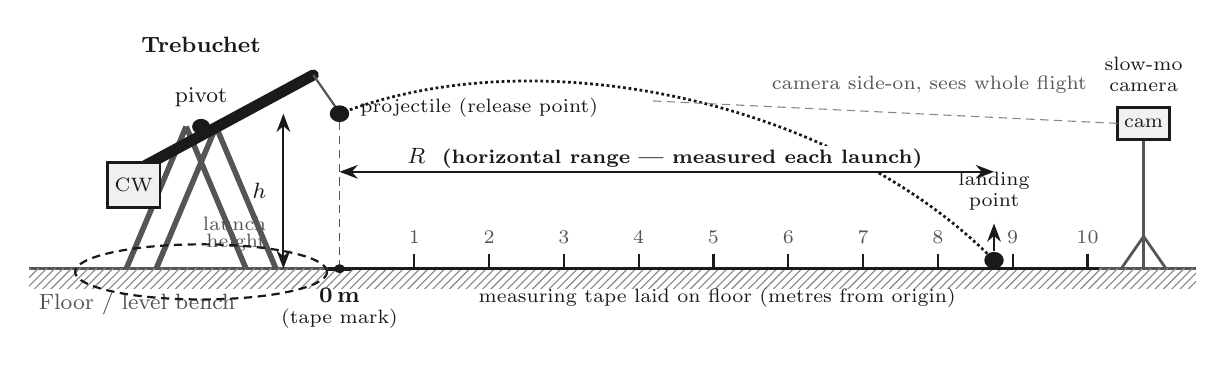
\begin{tikzpicture}[font=\footnotesize, x=0.95cm, y=0.82cm]

  % ===== FLOOR =====
  \draw[line width=1pt, LineGrey] (-0.3,0) -- (15.3,0);
  \fill[pattern=north east lines, pattern color=RuleGrey]
        (-0.3,-0.3) rectangle (15.3,0);
  \node[anchor=west, text=LineGrey] at (-0.3,-0.55) {Floor / level bench};

  % ===== TREBUCHET (left) =====
  % A-frame supports
  \draw[line width=2pt, LineGrey] (1.0,0) -- (1.8,2.2);
  \draw[line width=2pt, LineGrey] (2.6,0) -- (1.8,2.2);
  \draw[line width=2pt, LineGrey] (1.4,0) -- (2.2,2.2);
  \draw[line width=2pt, LineGrey] (3.0,0) -- (2.2,2.2);
  % pivot axle
  \fill[Ink] (2.0,2.2) circle (0.12);
  \node[anchor=south, text=Ink] at (2.0,2.35) {pivot};
  % throwing arm (counterweight low-left, sling end high-right)
  \draw[line width=4pt, Ink, line cap=round] (1.1,1.5) -- (3.5,3.0);
  % counterweight
  \draw[line width=1pt, Ink, fill=BoxGrey] (0.75,0.95) rectangle (1.45,1.65);
  \node[text=Ink] at (1.1,1.3) {\scriptsize CW};
  % sling + projectile
  \draw[line width=0.8pt, LineGrey] (3.5,3.0) -- (3.8,2.5);
  \fill[Ink] (3.85,2.4) circle (0.13);
  \node[anchor=west, text=Ink] at (4.0,2.5) {\scriptsize projectile (release point)};
  \node[anchor=south, text=Ink] at (2.0,3.2) {\bfseries Trebuchet};

  % ===== PLUMB LINE down to origin =====
  \draw[densely dashed, LineGrey] (3.85,2.27) -- (3.85,0);
  \fill[Ink] (3.85,0) circle (0.07);
  \draw[line width=1.5pt, Ink] (3.7,0) -- (4.0,0);
  \node[anchor=north, text=Ink, align=center] at (3.85,-0.15)
        {\bfseries 0\,m\\[-2pt]\scriptsize (tape mark)};

  % ===== HEIGHT h dimension =====
  \draw[{Stealth}-{Stealth}, line width=0.8pt, Ink] (3.1,0) -- (3.1,2.4);
  \node[anchor=east, text=Ink] at (3.0,1.2)
        {\bfseries $h$};
  \node[anchor=east, text=LineGrey, align=right] at (3.0,0.7)
        {\scriptsize launch};
  \node[anchor=east, text=LineGrey, align=right] at (3.0,0.4)
        {\scriptsize height};

  % ===== TRAJECTORY =====
  \draw[line width=1pt, Ink, densely dotted]
        (3.85,2.4) .. controls (6.5,3.6) and (10.5,2.6) .. (12.6,0.13);

  % ===== MEASURING TAPE =====
  \draw[line width=1.2pt, Ink] (3.85,0) -- (14.0,0);
  % tick marks every 1 m
  \foreach \x/\lab in {4.85/1,5.85/2,6.85/3,7.85/4,8.85/5,9.85/6,10.85/7,11.85/8,12.85/9,13.85/10}{
    \draw[line width=0.8pt, Ink] (\x,0) -- (\x,0.22);
    \node[anchor=south, text=LineGrey, font=\scriptsize] at (\x,0.24) {\lab};
  }
  \node[anchor=north, text=Ink] at (8.9,-0.15)
        {\scriptsize measuring tape laid on floor (metres from origin)};

  % ===== LANDING POINT =====
  \fill[Ink] (12.6,0.13) circle (0.13);
  \draw[{Stealth}-, line width=0.8pt, Ink] (12.6,0.7) -- (12.6,0.28);
  \node[anchor=south, text=Ink, align=center] at (12.6,0.75)
        {\scriptsize landing\\[-2pt]\scriptsize point};

  % ===== RANGE R dimension =====
  \draw[{Stealth}-{Stealth}, line width=0.8pt, Ink] (3.85,1.5) -- (12.6,1.5);
  \node[anchor=south, text=Ink, fill=white, inner sep=1pt] at (8.2,1.5)
        {\bfseries $R$ \;\scriptsize(horizontal range --- measured each launch)};

  % ===== CAMERA =====
  \draw[line width=1pt, LineGrey] (14.6,0) -- (14.6,2.0);
  \draw[line width=1pt, LineGrey] (14.3,0) -- (14.6,0.5) -- (14.9,0);
  \draw[line width=1pt, Ink, fill=BoxGrey] (14.25,2.0) rectangle (14.95,2.5);
  \node[text=Ink, font=\scriptsize] at (14.6,2.25) {cam};
  \node[anchor=south, text=Ink, align=center] at (14.6,2.6)
        {\scriptsize slow-mo\\[-2pt]\scriptsize camera};
  % camera sight line
  \draw[densely dashed, RuleGrey] (14.25,2.25) -- (8.0,2.6);
  \node[text=LineGrey, font=\scriptsize, anchor=west] at (9.5,2.85)
        {camera side-on, sees whole flight};

  % ===== EXCLUSION ZONE =====
  \draw[densely dashed, line width=0.8pt, Ink]
        (2.0,-0.05) ellipse (1.6cm and 0.35cm);
  \node[text=Ink, font=\scriptsize, anchor=north] at (1.0,-0.5) {};

\end{tikzpicture}
\end{center}

\vspace{-2pt}
{\footnotesize\color{LineGrey}
\textbf{Key:}\;
$h$ = vertical height from projectile release point to floor (measured once, fixed).\;
$R$ = horizontal distance from the ``0\,m'' origin to where the projectile lands (measured each launch).\;
The camera films side-on so students can count video frames to find the time of flight.}

\vspace{4pt}
{\color{RuleGrey}\rule{\linewidth}{0.8pt}}
{\footnotesize
\textbf{Notes / queries for teacher:} \underline{\hspace{7.5cm}}
\hfill \textbf{Prepared by (tech):} \underline{\hspace{3.5cm}}}

\end{document}
